\section{Observations}
	\subsection{180 degree Data}
		In figure \hyperref[obs:180cal]{Fig 3} we can see the calibration information for mapping the channels to appropriate enrgies. In \hyperref[obs:180blue]{Fig 4} and \hyperref[obs:180red]{Fig 5} we can see the coincident counts from the two sensors. Finally in \hyperref[obs:180]{Fig 6} we can see the analysis data about the observation.
		\begin{figure}[H]
			\centering
			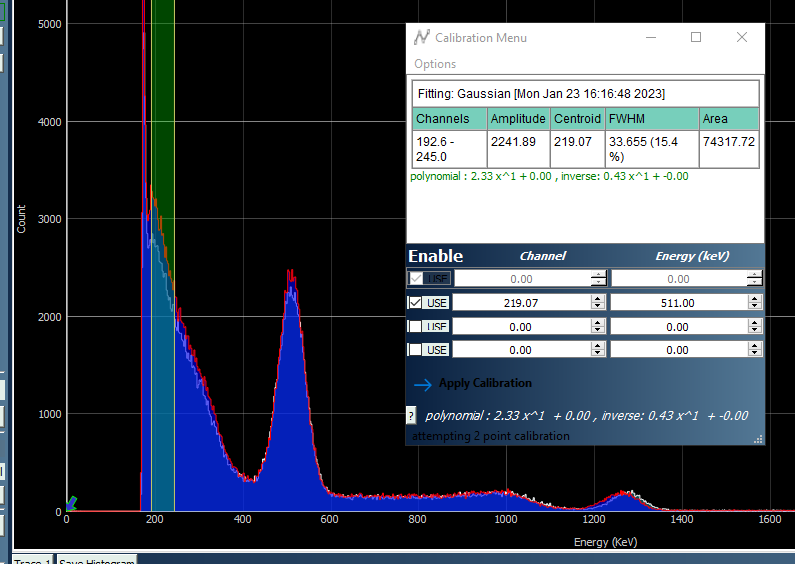
\includegraphics[width=0.7\columnwidth, height=3cm]{images/180_cal.png}
			\caption{$180^\circ$ calibration}
			\label{obs:180cal}
		\end{figure}
		\begin{figure}[H]
			\centering
			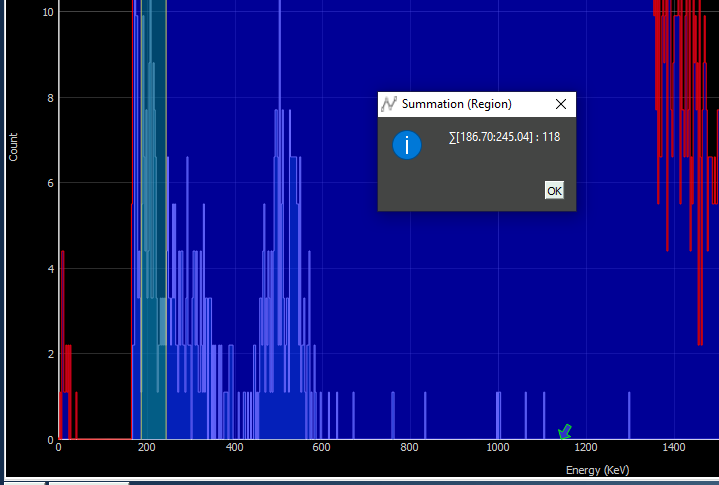
\includegraphics[width=0.7\columnwidth, height=3cm]{images/180blue.png}
			\caption{$180^\circ$ blue count}
			\label{obs:180blue}
		\end{figure}
		\begin{figure}[H]
			\centering
			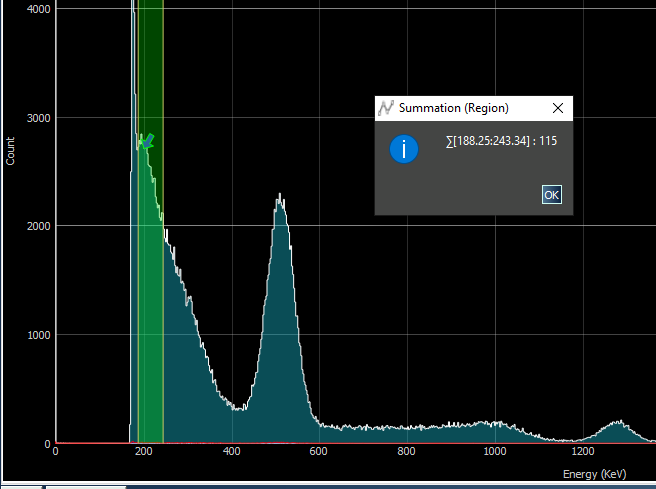
\includegraphics[width=0.7\columnwidth, height=3cm]{images/180red.png}
			\caption{$180^\circ$ red count}
			\label{obs:180red}
		\end{figure}
		\begin{figure}[H]
			\centering
			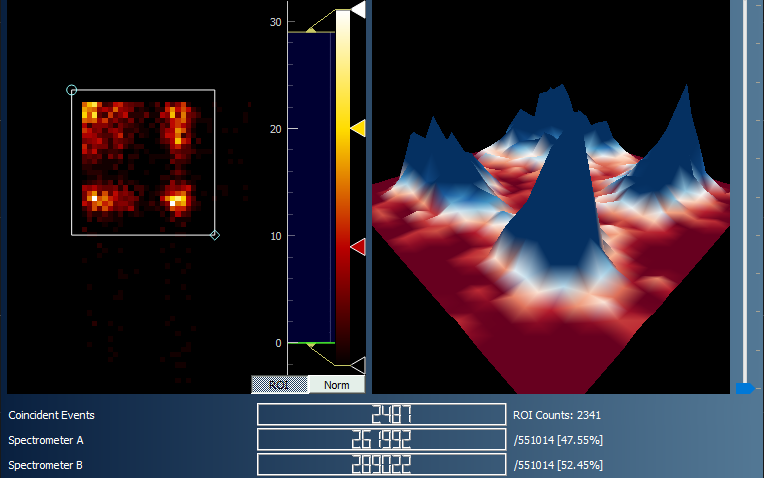
\includegraphics[width=0.7\columnwidth, height=3cm]{images/180.png}
			\caption{$180^\circ$ analysis}
			\label{obs:180}
		\end{figure}

	\subsection{175 degree Data}
		In figure \hyperref[obs:175cal]{Fig 7} we can see the calibration information for mapping the channels to appropriate enrgies. In \hyperref[obs:175blue]{Fig 8} and \hyperref[obs:175red]{Fig 9} we can see the coincident counts from the two sensors. Finally in \hyperref[obs:175]{Fig 10} we can see the analysis data about the observation.
		\begin{figure}[H]
			\centering
			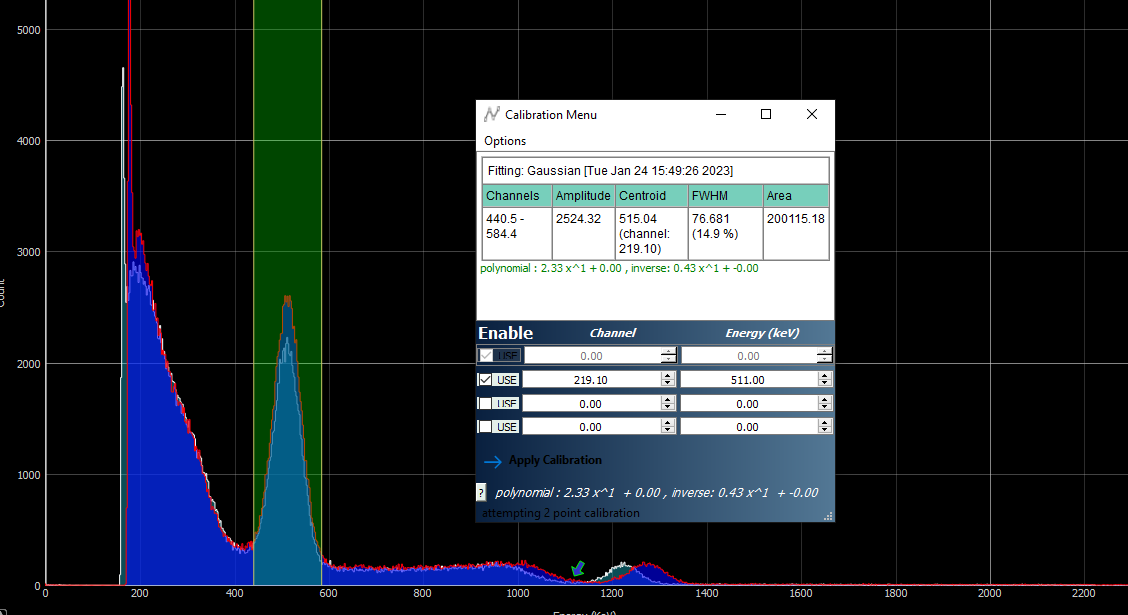
\includegraphics[width=0.7\columnwidth, height=3cm]{images/175_cal.png}
			\caption{$175^\circ$ calibration}
			\label{obs:175cal}
		\end{figure}
		\begin{figure}[H]
			\centering
			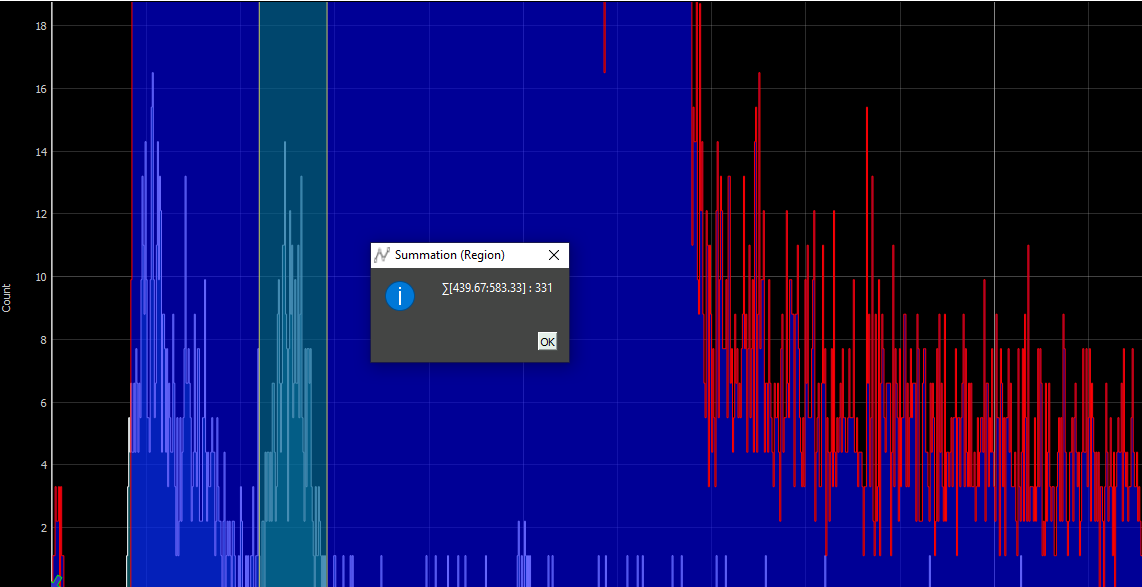
\includegraphics[width=0.7\columnwidth, height=3cm]{images/175blue.png}
			\caption{$175^\circ$ blue count}
			\label{obs:175blue}
		\end{figure}
		\begin{figure}[H]
			\centering
			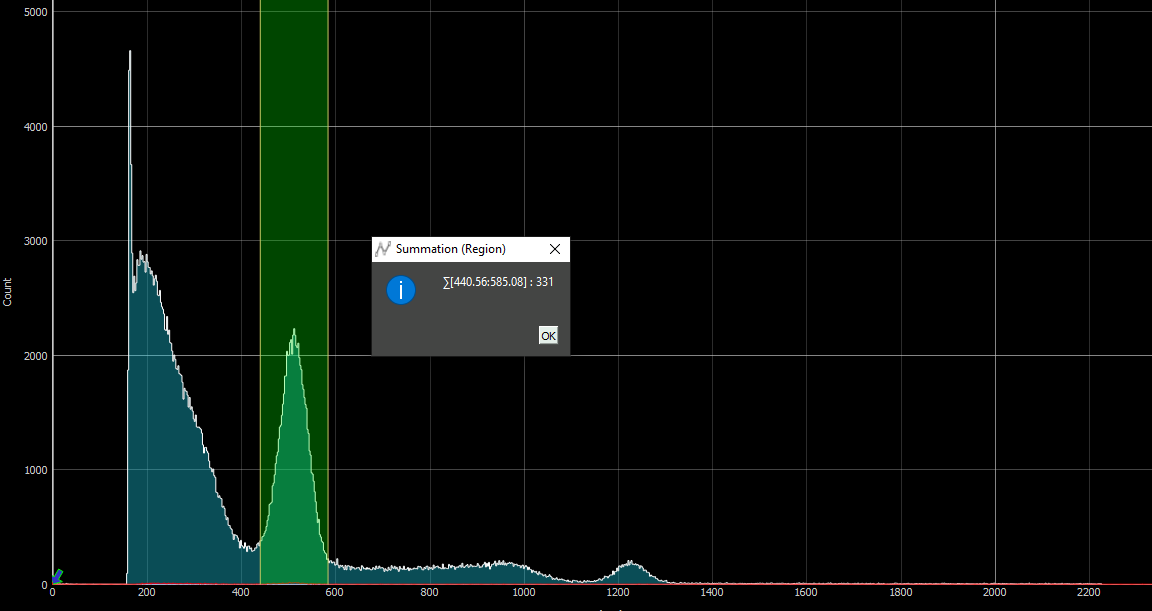
\includegraphics[width=0.7\columnwidth, height=3cm]{images/175red.png}
			\caption{$175^\circ$ red count}
			\label{obs:175red}
		\end{figure}
		\begin{figure}[H]
			\centering
			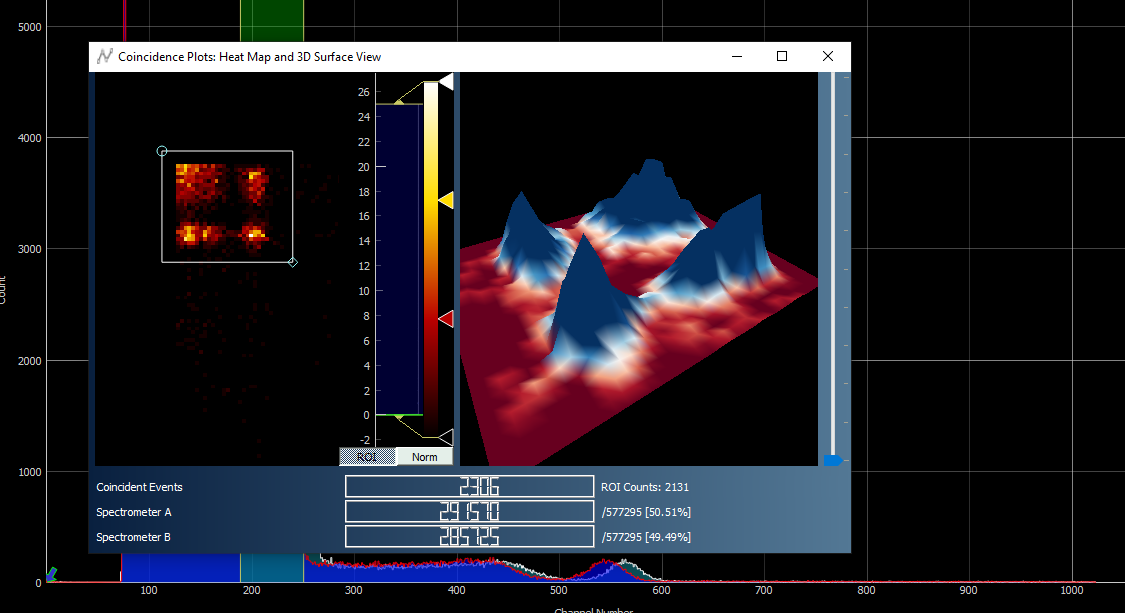
\includegraphics[width=0.7\columnwidth, height=3cm]{images/175.png}
			\caption{$175^\circ$ analysis}
			\label{obs:175}
		\end{figure}

	\subsection{185 degree Data}
		In figure \hyperref[obs:185cal]{Fig 11} we can see the calibration information for mapping the channels to appropriate enrgies. In \hyperref[obs:185blue]{Fig 12} and \hyperref[obs:185red]{Fig 13} we can see the coincident counts from the two sensors. Finally in \hyperref[obs:185]{Fig 14} we can see the analysis data about the observation.
		\begin{figure}[H]
			\centering
			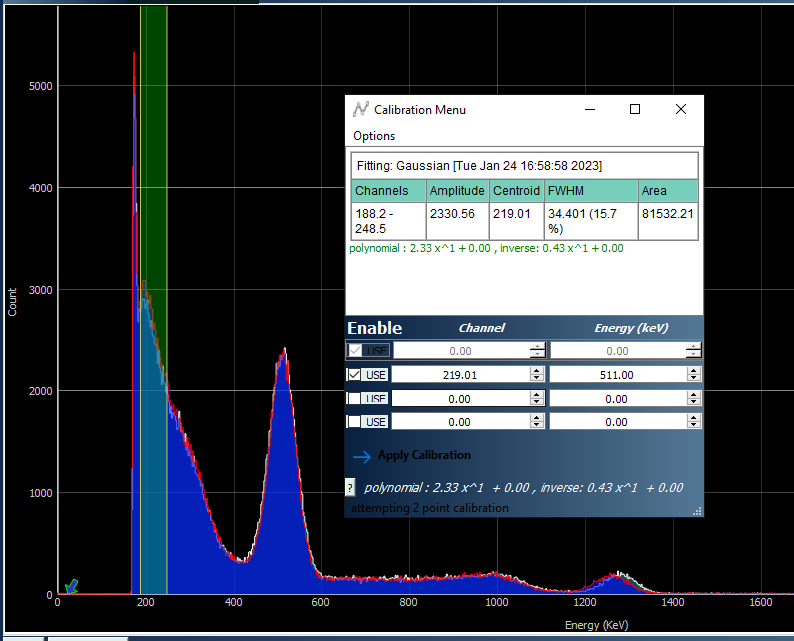
\includegraphics[width=0.7\columnwidth, height=3cm]{images/185_cal.png}
			\caption{$185^\circ$ calibration}
			\label{obs:185cal}
		\end{figure}
		\begin{figure}[H]
			\centering
			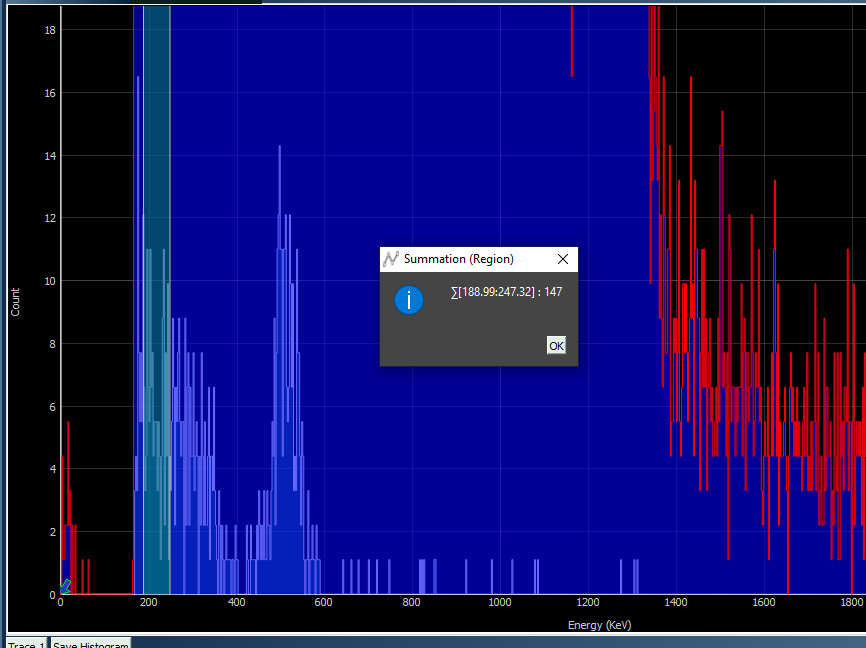
\includegraphics[width=0.7\columnwidth, height=3cm]{images/185blue.png}
			\caption{$185^\circ$ blue count}
			\label{obs:185blue}
		\end{figure}
		\begin{figure}[H]
			\centering
			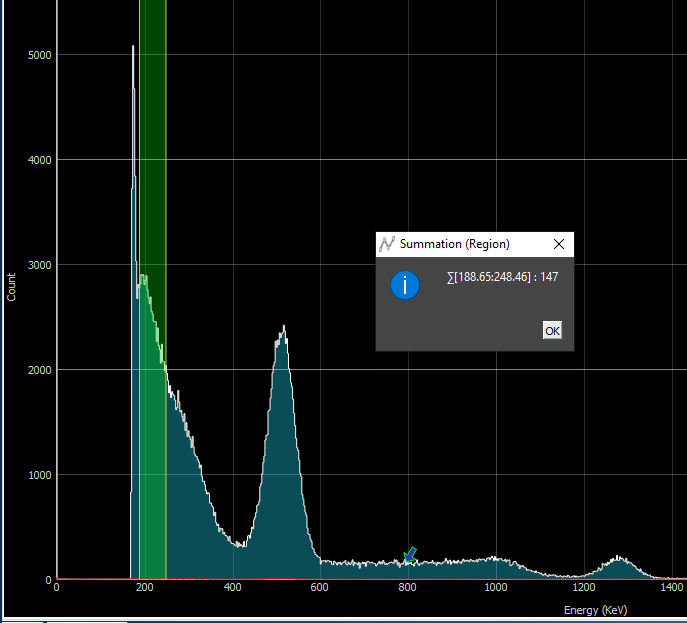
\includegraphics[width=0.7\columnwidth, height=3cm]{images/185red.png}
			\caption{$185^\circ$ red count}
			\label{obs:185red}
		\end{figure}
		\begin{figure}[H]
			\centering
			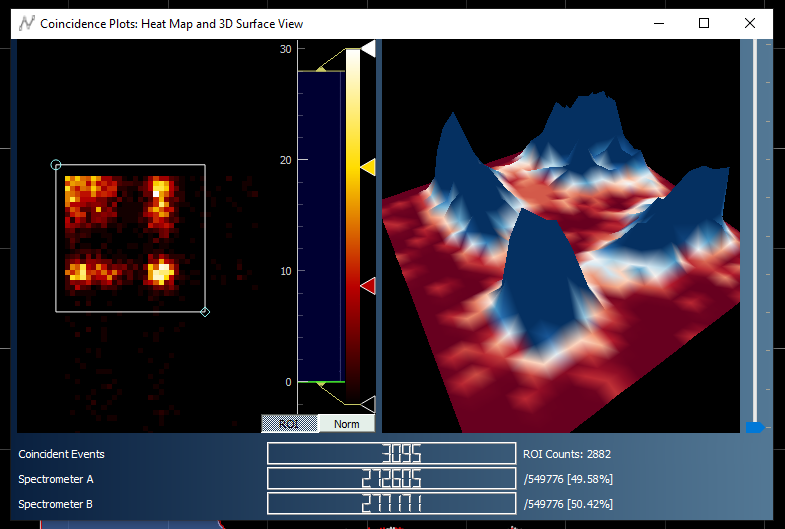
\includegraphics[width=0.7\columnwidth, height=3cm]{images/185.png}
			\caption{$185^\circ$ analysis}
			\label{obs:185}
		\end{figure}

	\subsection{90 degree Data}
		In figure \hyperref[obs:90cal]{Fig 15} we can see the calibration information for mapping the channels to appropriate enrgies. In \hyperref[obs:90blue]{Fig 16} and \hyperref[obs:90red]{Fig 17} we can see the coincident counts from the two sensors. Finally in \hyperref[obs:90]{Fig 18} we can see the analysis data about the observation.
		\begin{figure}[H]
			\centering
			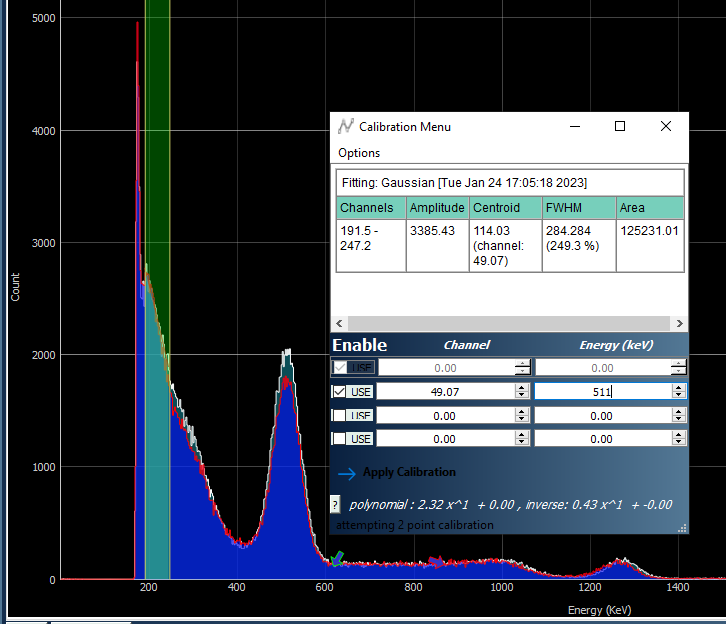
\includegraphics[width=0.7\columnwidth, height=3cm]{images/90_cal.png}
			\caption{$90^\circ$ calibration}
			\label{obs:90cal}
		\end{figure}
		\begin{figure}[H]
			\centering
			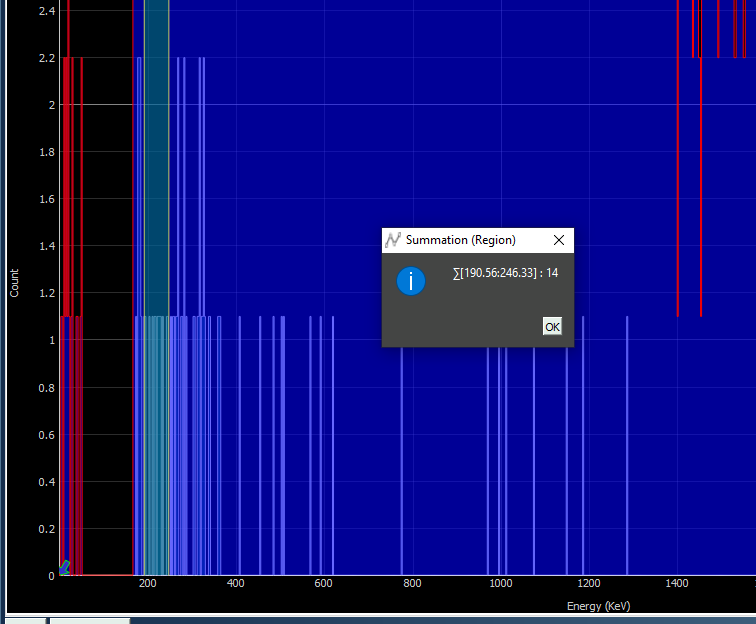
\includegraphics[width=0.7\columnwidth, height=3cm]{images/90blue.png}
			\caption{$90^\circ$ blue count}
			\label{obs:90blue}
		\end{figure}
		\begin{figure}[H]
			\centering
			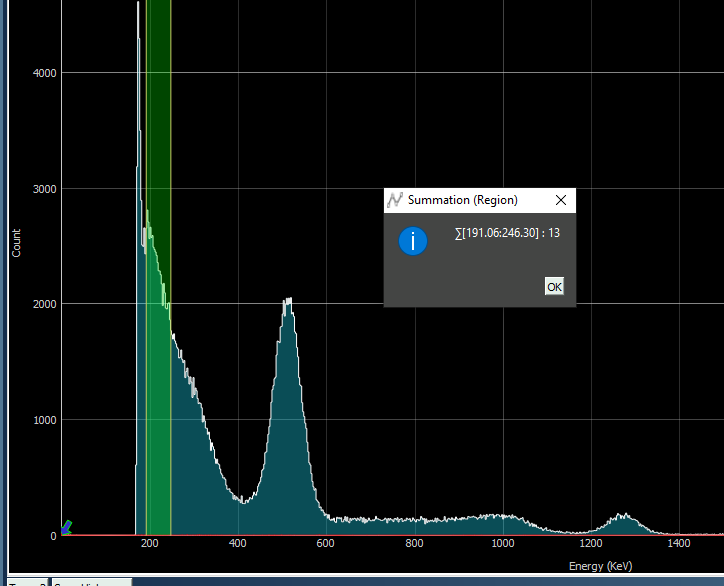
\includegraphics[width=0.7\columnwidth, height=3cm]{images/90red.png}
			\caption{$90^\circ$ red count}
			\label{obs:90red}
		\end{figure}
		\begin{figure}[H]
			\centering
			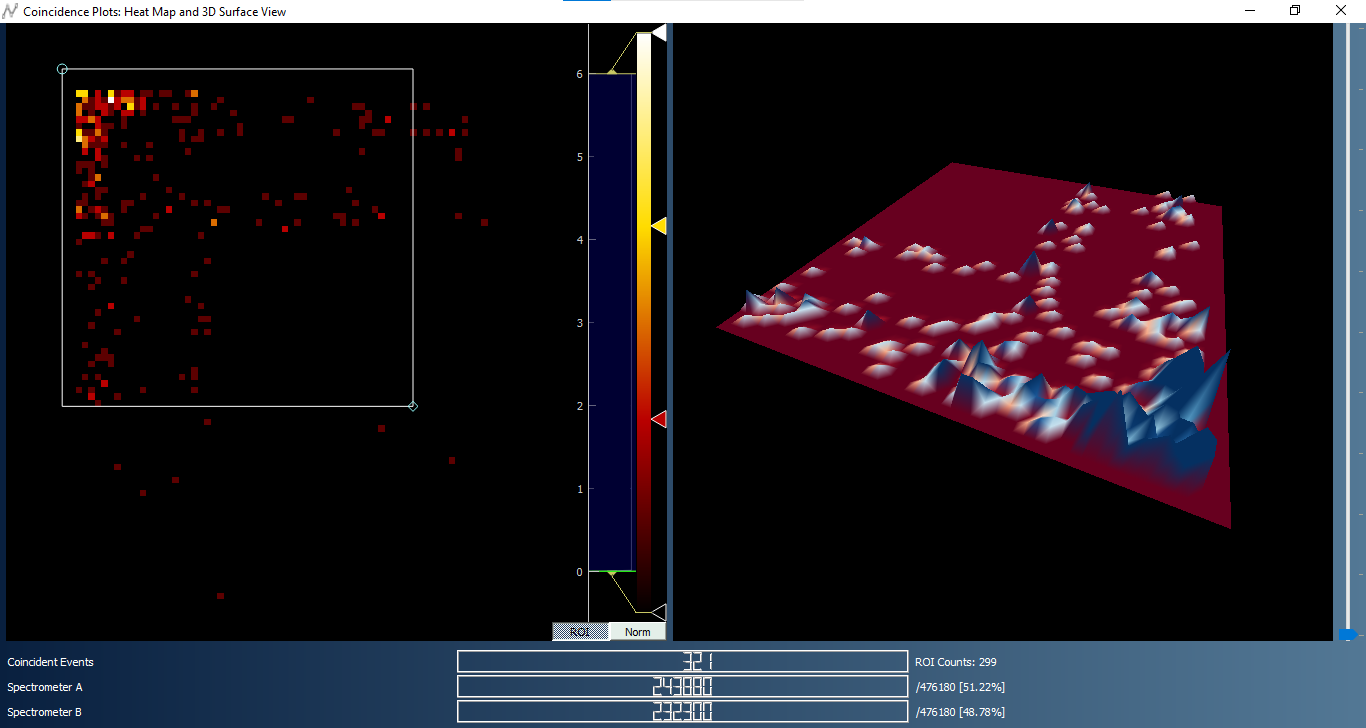
\includegraphics[width=0.7\columnwidth, height=3cm]{images/90.png}
			\caption{$90^\circ$ analysis}
			\label{obs:90}
		\end{figure}
